\subsection{Tổng quan tập dữ liệu}

Tổng điều tra xã hội (GSS) của Mỹ là một khảo sát xã hội học được tạo ra vào năm 1972 bởi Trung tâm Nghiên cứu Ý kiến Quốc gia (NORC) tại Đại học Chicago và được tài trợ bởi Quỹ Khoa học Quốc gia. 
GSS thu thập thông tin sáu tháng một lần và lưu giữ hồ sơ lịch sử về nhân khẩu học, các mối quan tâm, trải nghiệm, thái độ của cư dân Hoa Kỳ. Đây là một trong những nghiên cứu có ảnh hưởng nhất trong khoa học xã hội và thường được nhắc đến trong các ấn phẩm hàng đầu, bao gồm The New York Times, The Wall Street Journal và Associated Press.

Bài toán hiện tại nghiên cứu dữ liệu về hình thức làm việc của một người Mỹ trưởng thành vào năm 2016. 
Trong đó, mục tiêu hướng tới là xem xét những yếu tố sử dụng mạng xã hội là "snapchat" và "instagram" có quyết định đến hình thức làm việc của một người hay không.

Dữ liệu được trích xuất từ tập dữ liệu GSS và có cấu trúc dạng bảng. Mỗi hàng trong bảng đại diện cho một cá nhân được khảo sát trong nghiên cứu.

\begin{itemize}
    \item Số lượng quan sát: 2867 quan sát
    \item Số lượng biến: 9 biến
\end{itemize}

Dưới đây là mô tả chi tiết về ý nghĩa các cột trong tập dữ liệu dựa trên quan sát và phân tích các biến:

\begin{itemize}
    \item harass5: Biến này là kết quả của một câu hỏi về việc có bị quấy rối (harassment) trong năm 2016 hay không. 
    Giá trị 'No' có thể chỉ ra rằng người nghiên cứu không bị quấy rối, và giá trị khác, chẳng hạn 'Yes', có thể chỉ ra ngược lại. Giá trị "Does not apply (i do not have a job/superior/co-worker)" cho thấy rằng người tham gia khảo sát không có công việc, người cấp trên hoặc đồng nghiệp, nên họ không áp dụng được tình huống này vào tình hình làm việc của họ.
    \item emailmin: Thời gian trung bình hàng ngày dành cho email (được tính bằng phút).
    \item emailhr: Số giờ hàng ngày dành cho email.
    \item educ: Mức học vấn của người nghiên cứu, có thể là số năm học.
    \item polviews: Quan điểm chính trị (political views) của người nghiên cứu là biến phân loại, gồm các giá trị: "Conservative", "Moderate", "Liberal", "Slightly conservative", "Slightly liberal".
    \item advfront: Quan điểm về tiến bộ (advancement) trong công việc là biến phân loại, gồm các giá trị: "Strongly agree", "Agree", "Neutral", "Disagree", "Strongly disagree", "Dont know".
    \item snapchat: Có sử dụng ứng dụng Snapchat không (có thể là "Yes" hoặc "No").
    \item instagrm: Có sử dụng ứng dụng Instagram không (có thể là "Yes" hoặc "No").
    \item wrkstat: Tình trạng làm việc (work status) của người nghiên cứu là biến phân loại, gồm các giá trị: "Working fulltime", "Working parttime", "Retired", "Unemployed", "Unempl, laid off", "School", “Other”, "Temp not working".
\end{itemize}

\begin{figure}[h!]
    \centering
    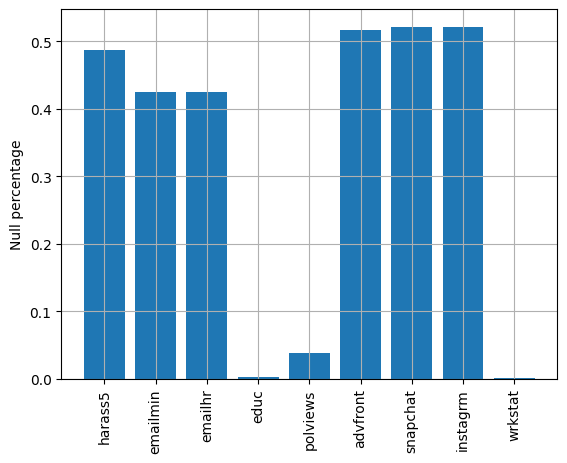
\includegraphics[width=0.6\textwidth]{figures/Thanh/Data_Analysis/null_percentage_columns.png}
    \caption{Số lượng quan sát có giá trị null trong từng biến}
    \label{fig:null_percentage_columns}
\end{figure}

Hình \ref{fig:null_percentage_columns} thể hiện số lượng giá trị null trong từng biến. Từ hình \ref{fig:null_percentage_columns}, ta rút ra được nhận xét rằng hầu hết các biến của tập dữ liệu đều có các giá trị null.

Trong đó, 3 biến "advfront", "snapchat" và "instagram" có nhiều giá trị null nhất và 2 biến "educ" và "wrkstat" có ít giá trị null nhất, chi tiết trong Bảng \ref{tab:null-percentage} dưới.

\begin{table}[h!]
    \centering
    \resizebox{\columnwidth}{!}{
        \begin{tabular}{|l|c|c|c|c|c|c|c|c|c|}
            \hline
            & harass5 & emailmin & emailhr & educ & polviews & advfront & snapchat & instagram & wrkstat \\
            \hline
            Giá trị null & 1398 & 1218 & 1218 & 9 & 111 & 1482 & 1495 & 1495 & 3 \\
            \hline
            Giá trị khác rỗng & 1469 & 1649 & 1649 & 2858 & 2756 & 1385 & 1372 & 1372 & 2864 \\
            \hline
            Tỷ lệ giá trị null (\%) & 48.7\% & 42.4\% & 42.4\% & 0.3\% & 3.8\% & 51.7\% & 52.1\% & 52.1\% & 0.1\% \\
            \hline
        \end{tabular}
    }
    \caption{Tỷ lệ giá trị null trong từng cột}
    \label{tab:null-percentage}
\end{table}

Ta xử lý hai cột "emailmin" và "emailhr" bằng cách tạo ra một cột mới "emailtotal" bằng công thức 60 x "emailhr" + "emailmin".
Đối với các cột là dạng biến phân loại (categorical), các giá trị null ta sẽ tạo ra một giá trị mới là "Unknown".
Riêng đối với cột "emailtotal" là biến định lượng, số lượng các giá trị null quá nhiều ta sẽ phải tách ra làm hai tập dữ liệu riêng.
Một tập dữ liệu chỉ bao gồm các quan sát có cột "emailtotal" không phải giá trị null và một tập dữ liệu chỉ bao gồm quan sát có cột "emailtotal" là giá trị null.

\textbf{Phân tích mô tả tập dữ liệu về Tình trạng làm việc dựa trên yếu tố sử dụng mạng xã hội là "snapchat" và "instagram".}:

Mỗi cá nhân trong nghiên cứu (ngoài các các nhân không có dữ liệu ở biến này) sẽ thuộc một trong 8 tình trạng việc làm khác nhau.  Dựa trên yếu tố cá nhân đó có sử dụng mạng xã hội là “snapchat” và “instagram” hay không, ta có bảng thống kê chi tiết như sau:

\begin{table}[h!]
    \centering
    \resizebox{\columnwidth}{!}{
        \begin{tabular}{|l|c|c|c|c|c|}
            \hline
            \thead{Tình trạng việc làm \\ (wrkstat)} & \thead{Số lượng \\ quan sát} & \thead{Số lượng quan sát \\ (Có sử dụng instagram)} & \thead{Tỷ lệ sử dụng \\ instagram} & \thead{Số lượng quan sát \\ (Có sử dụng snapchat)} & \thead{Tỷ lệ sử dụng \\ snapchat} \\
            \hline
            Working fulltime &1321 &219 & 16.5\% &159 &12.0\%  \\
            \hline
            Retired & 574 & 12 & 2.0\% & 8 & 1.3\% \\
            \hline
            Working partime &345 &0 &0.0\% &0 & 0.0\% \\
            \hline
            Keeping house & 284 & 43 & 15.1\% & 22 & 7.7\% \\
            \hline
            Unempl, laid off & 118 & 23 & 19.5\% & 18 & 15.2\% \\
            \hline
            Other & 89 & 4 & 4.4\% & 5 & 5.6\% \\
            \hline
            School & 76 & 21 & 27.6\% & 21 & 27.6\% \\
            \hline
            Temp not working & 57 & 17 & 29.8\% & 11 & 19.2\% \\
            \hline
        \end{tabular}
    }
    \caption{ Tình trạng làm việc dựa trên yếu tố sử dụng mạng xã hội}
    \label{tab:work-status}
\end{table}

Từ bảng chi tiết trên, ta thấy:

\begin{itemize}
    \item Hai nhóm "School" và "Temp not working" tức đang đi học và nghỉ việc tạm thời có tỷ lệ sử dụng hai mạng xã hội Instagram và Snapchat cao nhất và cao hơn hẳn các nhóm còn lại.
    \item Mạng xã hội Instagram được nhiều người ưa thích sử dụng hơn vì hầu hết các nhóm tình trạng công việc thì tỷ lệ người sử dụng Instagram đều lớn hơn mạng xã hội Snapchat.
    \item Nhóm "Retired" tức nghỉ hưu có tỷ lệ sử dụng cả hai mạng xã hội đều rất thấp, có thể được lý giải bởi hai mạng xã hội này đều hướng tới người sử dụng trẻ.
\end{itemize}
